\documentclass[a4paper,12pt]{article}
\usepackage[T2A]{fontenc}
\usepackage[utf8]{inputenc}
\usepackage[english,russian]{babel}
\usepackage{circuitikz}
\usepackage{wrapfig}
\usepackage{makecell}
\usepackage{tabularx}
\usepackage{graphicx}
\usepackage{gensymb}
\usepackage{cancel} %cancel symbol
\usepackage{amsmath,amsfonts,amssymb,amsthm,mathtools}

%tikz (draw)

\usepackage{tikz}

%tikz libraries

\usetikzlibrary{intersections}
\usetikzlibrary{arrows.meta}
\usetikzlibrary{calc,angles,positioning}

\usepackage{float}

\parindent=0ex

\graphicspath{ {C:/Users/George/Documents/MIPT_TEX/LAB_1_2_5} }



\begin{document}
	

\begin{titlepage}
	\begin{center}
		МОСКОВСКИЙ ФИЗИКО-ТЕХНИЧЕСКИЙ ИНСТИТУТ (НАЦИОНАЛЬНЫЙ ИССЛЕДОВАТЕЛЬСКИЙ УНИВЕРСИТЕТ) \\
		
		
		\hfill \break
		Факультет обшей и прикладной физики\\
		\vspace{2.5cm}
		\large{\textbf{Отчёт по лабораторной работе 1.2.5 <<Исследование прецессии уравновешенного гороскопа>>}}\\
		\hfill \break
		\\
	\end{center}
	
	\begin{flushright}
		Выполнил:\\
		Студент гр. Б02-304\\
		Головинов. Г.А.
	\end{flushright}
	
	\vspace{7cm}
	
	\begin{center}
		
\includegraphics[width=0.15\linewidth]{uni}
	\end{center}
	

	

	\vfill
	
	\begin{center} Долгопрудный, 2023 \end{center}
	
	\thispagestyle{empty}
	
\end{titlepage}


	\newpage
	\pagenumbering{arabic}
	
	\section{Аннотация}
	\paragraph{Цель работы:} \hspace{-4mm} 
	исследовать вынужденную прецессию гироскопа; установить зависимость скорости вынужденной прецессии от величины момента сил, действующих на ось гироскопа; определить скорость вращения ротора гироскопа и сравнить ее со скоростью, рассчитанной по скорости прецессии.
	\paragraph{Используемые инструменты:} \hspace{-4mm} гироскоп в кардановом подвесе, секундомер, набор грузов, отдельный ротор гироскопа, цилиндр известной массы, крутильный маятник, штангенциркуль, линейка\\
	\section{Основные теоретические сведения}
	Уравнения движения твердого тела можно записать в виде
	
	\begin{equation}
		\label{dpdt}
		\frac{d\vec p}{dt}=\vec{F}
	\end{equation}
	\begin{equation}
		\label{dldt}
		\frac{d\vec{L}}{dt}=\vec{M}
	\end{equation}
	
	уравнение \eqref{dpdt} выражает закон движения центра масс тела, а \eqref{dldt} -- уравнение моментов. Этих двух уравнений достаточно для полного описания движения твердого тела, так как у него только шесть степеней свободы.\\
	
	Если сила $\vec{F}$ не зависит от угловой скорости, а момент $\vec{M}$ -- от скорости поступательного движения, то эти два уравнения можно рассматривать независимо друг от друга (то есть вращательное и поступательное движение не зависят друг от друга).\\
	
	Момент импульса $\vec{L}$ твердого тела в его главных осях $x,y,z$ равен
	\begin{equation}
		\label{L}
		\vec{L}=\vec{i}I_x\omega_x+\vec{j}I_y\omega_y+\vec{k}I_z\omega_z
	\end{equation}
	где $I_x, I_y, I_z$ -- моменты инерции относительно соответствующих осей, $\omega_x, \omega_y, \omega_z$ -- компоненты вектора угловой скорости $\vec{\omega}$. Если тело быстро вращается вокруг некоторой оси, например:
	\[
		I_z\omega_z \gg I_x\omega_x,\hspace{1mm} I_y\omega_y
	\]
	то такое тело принято называть гироскопом. Гироскоп называется уравновешенным, если его центр масс неподвижен.\\
	
	В силу \eqref{dldt} приращение момента импульса определяется интегралом
	\begin{equation}
		\label{intdL}
		\Delta\vec{L}=\int\vec{M}dt
	\end{equation}
	Если момент внешних сил действует в течение короткого промежутка времени, из интеграла \eqref{intdL} следует, что приращение $\Delta\vec{L}$ момента импульса заметно меньше самого момента импульса:
	\[
	|\vec{L}| \gg |\Delta\vec{L}|
	\]
	С этим связана замечательная устойчивость, которую приобретает движение гироскопа после приведения его в быстрое вращение.\\
	
	Чтобы определить, какие силы необходимо приложить к гироскопу, чтобы определенным способом изменить направление его оси, необходимо воспользоваться основным уравнением гироскопии:
	
	\begin{equation}
		\label{gyro}
		\vec{M}=[\vec{\Omega}|\vec{L}]
	\end{equation}
	где $\vec{\Omega}$ -- вектор угловой скорости прецессии гироскопа. Соответственно выбирая некоторое направление прецессии, мы можем найти направление момента силы, а отсюда найти направление и самой силы.\\
	
	Если $\vec{\Omega} \perp \vec{L}$, то можно найти $\Omega$ через момент силы $M$.
	
	\begin{equation}
		\label{Omega}
		\Omega=\frac{M}{I_z\omega_0\sin{\alpha}}=\frac{mgl\sin{\alpha}}{I_z\omega_0\sin{\alpha}}=\frac{mgl}{I_z\omega_0}
	\end{equation}
	где $m$ -- масса груза, $l$ -- расстояние от центра масс гироскопа до точки приложения силы, $I_z$ -- момент инерции ротора гироскопа относительно оси вращения, $\omega_0$ -- угловая скорость вращения гироскопа.\\
	
	Так как гироскоп в работе уравновешенный -- $l$ можно считать как расстояние от центра карданова подвеса до точки крепления груза.
	
	\begin{figure}
		\centering
		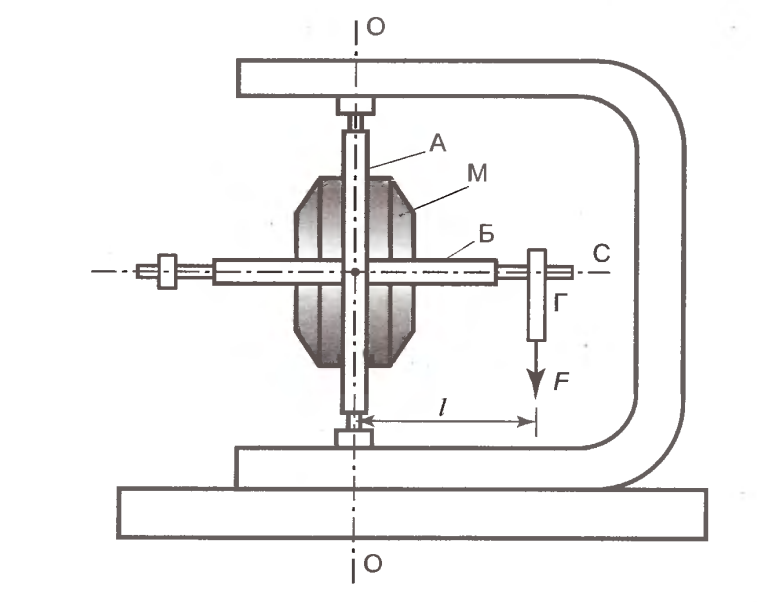
\includegraphics[width=0.7\linewidth]{fig1}
		\caption{Схема экспериментальной установки}
		\label{fig:fig1}
	\end{figure}
	
	В предыдущих вычислениях мы считали, что момент силы трения равен нулю. Если действие силы трения на ротор гироскопа компенсировано электромотором, то сила трения в подвесе никак не скомпенсирована. Если учесть действие этой силы, то гироскоп будет постепенно <<опускаться>> тем концом, на который подвешен груз. Момент силы трения можно определить из угловой скорости прецессии относительно другой оси. Момент силы трения можно вычислить из основного уравнения гироскопии следующим способом:
	
	\begin{equation}
		\label{Mfric}
		M_{fr}=I_0\omega_0\Omega_{fr}
	\end{equation}
	
	\paragraph{Измерение момента инерции ротора гироскопа}
	Момент инерции гироскопа относительно оси вращения мы найдем (аналогично работе 1.2.1) с помощью крутильных колебаний. Период крутильных колебаний зависит от момента инерции тела $I_0$ и модуля кручения проволоки $k$.
	\begin{equation}
		\label{T0}
		T_0=2\pi\sqrt{\frac{I_0}{k}}
	\end{equation}
	
	Для исключения модуля кручения необходимо подвесить цилиндр правильной формы с известными размерами и массой (то есть известным моментом инерции $I_1$). Тогда момент инерции ротора мы найдем из соотношения:
	\begin{equation}
		\label{I0}
		I_0=I_1\frac{T_0^2}{T_1^2}
	\end{equation}
	где $T_1$ -- период крутильных колебаний цилиндра.\\
	
	\paragraph{Измерение скорости вращения ротора гироскопа} Скорость вращения ротора можно найти не только с помощью прецессии: статор гироскопа имеет две обмотки. Обычно обе используются для ускорения ротора, однако в нашей работе только одна разгоняет ротор. Вторая используется для измерения числа оборотов ротора. Ротор электромотора всегда немного намагничен, из-за этого при каждом вращении на второй обмотке возникает переменная ЭДС индукции, частота которой равна частоте вращения ротора. Частоту этой ЭДС можно измерить с помощью фигур Лиссажу, получаемых на экране осциллографа, если на один вход подать искомую ЭДС, а на другой -- переменное напряжение известной частоты. При совпадении частот на экране должен появиться неподвижный эллипс.
	
	\section{Методика измерений}
	
	Работа сводится к нескольким простым задачам:
	нужно найти угловую скорость прецессии в зависимости от момента силы тяжести груза, если теория верна, то мы получим прямую с коэффициентом наклона равной $L^{-1}$\\
	
	Для того, чтобы это подтвердить необходимо измерить момент инерции ротора гироскопа и угловую скорость его вращения. Это и будут две оставшиеся подзадачи этой работы.
	
	
	\section{Результаты измерений и их обработка}
	
	Сначала требуется узнать точные массы предоставленных нам грузов. Несмотря на то, что на них уже есть маркировка, чтобы получить более точный результат, масса каждого из них была повторно измерена.
	
	\begin{table}[H]
		\centering
		\small
		\begin{tabular}{|c|c|c|c|c|c|c|c|c|c|c|}
			\hline
			$n$ & 1 & 2 & 3 & 4 & 5 & 6 & 7 & 8 & 9 & 10 \\
			\hline
			$m$, g & 60.6 & 76.5 & 92.5 & 115.9 & 141.5 & 141.5 & 173.0 & 214.6 & 269.4 & 339.9 \\
			\hline
		\end{tabular}
		\caption{Полученные массы грузов}
	\end{table}
	
	Для каждого из девяти грузов измерим время, за которое гироскоп совершит один полный оборот, а также угол на который ось гироскопа опустилась. В каждом опыте начальный угол наклона гироскопа от горизонтали был выбран $+6\degree$, так как его можно считать малым.
	
	\begin{table}[H]
		\centering
		\begin{tabular}{|c|c|c|c|c|c|c|}
			\hline
			$N$ & $m$, g & $T$, s & $\Omega$, rad/s & $\Delta\alpha\degree$ & $\Delta\alpha$, rad & $\dot{\alpha}$, rad/s \\
			\hline
			1 & 60.6 & 169 & 0.037 & 12.0 & 0.21 & 0.0012 \\
			\hline
			2 & 76.5 & 131 & 0.048 & 8.9 & 0.15 & 0.0012 \\
			\hline
			3 & 92.5 & 109 & 0.058 & 4.9 & 0.08 & 0.0008 \\
			\hline
			4 & 115.9 & 87 & 0.072 & 6.0 & 0.10 & 0.0012 \\
			\hline
			5 & 141.5 & 72 & 0.087 & 3.9 & 0.07 & 0.0010 \\
			\hline
			5 & 141.5 & 71 & 0.088 & 3.1 & 0.05 & 0.0008 \\
			\hline
			5 & 141.5 & 71 & 0.088 & 3.9 & 0.07 & 0.0010 \\
			\hline
			6 & 173 & 58 & 0.108 & 2.3 & 0.04 & 0.0007 \\
			\hline
			7 & 214.6 & 48 & 0.132 & 2.0 & 0.03 & 0.0007 \\
			\hline
			8 & 269.4 & 37 & 0.168 & 2.0 & 0.03 & 0.0009 \\
			\hline
			9 & 339.9 & 31 & 0.206 & 1.4 & 0.02 & 0.0008 \\
			\hline
		\end{tabular}
		\caption{Результаты измерений для всех девяти грузов}
	\end{table}
	
	Для пятого груза было проведено 3 измерения, чтобы оценить случайную погрешность наших измерений. Как видно, время (следовательно и угловая скорость прецессии) получаются достаточно точно, а вот угол, на который ось гироскопа опустилась, сильно меняется от измерения к измерению. Да и в целом, из теории мы ожидаем увидеть некую линейную (возможно квадратичную) зависимость, а наши результаты точно не образуют кривую.\\
	
	\paragraph{Результаты измерений угловой скорости вращения ротора} С помощью осциллографа и цифрового генератора частот была получена частота $\omega_0=400.017 hz$, ее погрешность мы оценим в $0.005 hz$, так как точность измерений этим способом достаточно велика.\\
	
	\paragraph{Результаты измерений момента инерции ротора}
	
	Момент инерции цилиндра $I_1 = 0.00123 \pm 0.00006$ кг$\cdot$м$^2$
	
	Погрешность измерения момента инерции цилиндра будем вычислять по формуле:
	\begin{equation}
		\label{sigmaI}
		\sigma_I=I\sqrt{\left(2\frac{\sigma_r}{r}\right)^2 + \left(\frac{\sigma_m}{m}\right)^2}
	\end{equation}
	
	Период колебаний ротора:
	
	\begin{table}[H]
		\centering
		\begin{tabular}{|c|c|c|c|}
			\hline
			$n$ & 1 & 2 & 3 \\
			\hline
			$t$, s & 31.7 & 31.8 & 31.8 \\
			\hline
			$N$ & 10 & 10 & 10 \\
			\hline
			$T$, s & 3.17 & 3.18 & 3.18 \\
			\hline
		\end{tabular}
		\caption{Результаты измерения периода крутильных колебаний ротора}
	\end{table}
	
	Стандартное отклонение $\sigma_T = 0.0006$ s. Этой погрешностью можно пренебречь, оставим лишь систематическую погрешность $\sigma_T=0.02$ s из расчета, что средняя реакция человека равна $0.2$ s.
	
	Период колебаний цилиндра:
	
	\begin{table}[H]
		\centering
		\begin{tabular}{|c|c|c|c|}
			\hline
			$n$ & 1 & 2 & 3 \\
			\hline
			$t$, s & 40.2 & 40.0 & 40.0 \\
			\hline
			$N$ & 10 & 10 & 10 \\
			\hline
			$T$, s & 4.02 & 4.00 & 4.00 \\
			\hline
		\end{tabular}
		\caption{Результаты измерений периода крутильных колебаний цилиндра}
	\end{table}
	
	Стандартное отклонение $\sigma_T = 0.01$ s, этим значением опять пренебрежем, будем считать погрешность $\sigma_T$ равной $0.02$ s.\\
	
	Тогда по формуле \eqref{I0} найдем момент инерции ротора:
	
	\[
		I_0=(0.00077\pm 0.00009) \text{кг}\cdot\text{м}^2
	\]
	
	Погрешность момента инерции ротора вычисляем по формуле
	
	\begin{equation}
		\label{sigmaI0}
		\sigma_{I_0}=I_0\sqrt{\left(\frac{\sigma_{I_1}}{I_1}\right)^2+ \left(\frac{2\sigma_{T_0}}{T_0}\right)^2+\left(\frac{2\sigma_{T_1}}{T_1}\right)^2}
	\end{equation}
	
	Тогда момент импульса $L=I_0\omega_0=I_02\pi\nu$ получится $L=1.94\pm 0.22$ кг$\cdot$м$^2$
	
	\paragraph{Измерение момента импульса с помощью коэффициента наклона графика $\Omega(M)$}
	
	Из таблицы 2 возьмем значения $\Omega$ и $mgl$ при $l = 0.122$ m, чтобы построить зависимость $\Omega(M)=\Omega(mgl)$\\
	
	\begin{figure}[H]
		\centering
		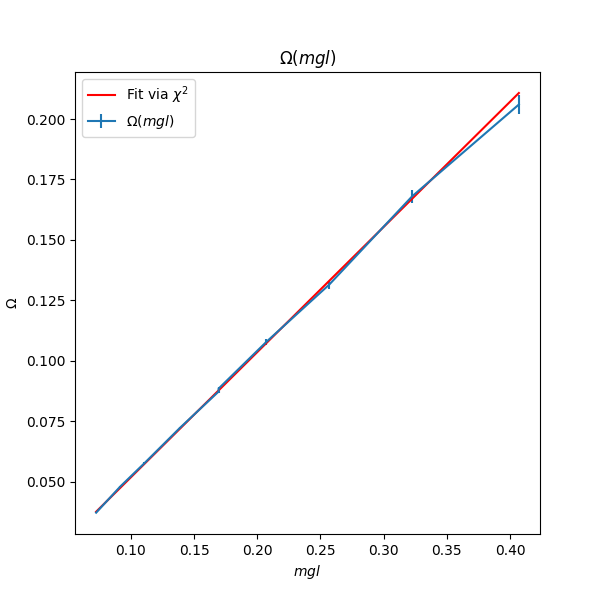
\includegraphics[width=0.7\linewidth]{fig2}
		\caption{Зависимость угловой скорости прецессии от момента силы тяжести груза}
		\label{fig:fig2}
	\end{figure}
	
	Аппроксимируя по методу $\chi^2$ получим $k = 0.5178$, откуда $L = 1.93$ кг$\cdot$м$^2$ (погрешность пренебрежимо мала)
	
	\paragraph{Расчет момента силы трения}
	
	По формуле \eqref{Mfric} вычисляем момент силы трения для каждого груза. 
	
	\begin{figure}[H]
		\centering
		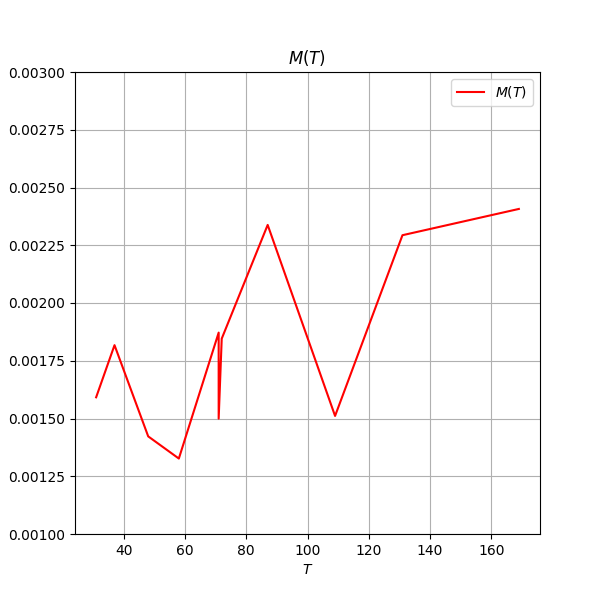
\includegraphics[width=0.7\linewidth]{fig3}
		\caption{Зависимость момента силы трения от периода прецессии}
		\label{fig:fig3}
	\end{figure}
	
	Видно, что шум в данных не дает возможности чем-то фитировать эту зависимость. Кроме того, мы ожидали либо горизонтальную прямую (в случае сухого трения), либо линейную зависимость с отрицательным коэффициентом наклона (в случае вязкого трения). А тут можно увидеть обратное.
	
	\section{Обсуждение результатов и выводы}
	В результате выполнения работы мы познакомились с явлением прецессии гироскопа. Получили экспериментально зависимость угловой скорости прецессии от момента силы тяжести груза, из которой по методу $\chi^2$ нашли значение момента импульса ротора гироскопа. Эту же величину мы получили другим способом: измерив момент инерции ротора гироскопа и частоту его вращения. Полученные результаты очень хорошо друг с другом соотносятся.\\
	
	Подобное нельзя сказать про зависимость момента силы трения от периода прецессии. Зависимость получилась шумная, по ней сложно сделать выводы. Это может быть связано в том числе с тем, что наш гироскоп был не совсем сбалансирован -- при длительном отсутствии воздействия груза, гироскоп все равно прецессирует. Это может говорить о неправильной балансировке. Кроме того, на результат повлияло отсутствие удобной шкалы для определения угла, на который гироскоп опускается.
	
\end{document}